\begin{figure}[h]
	\centering
	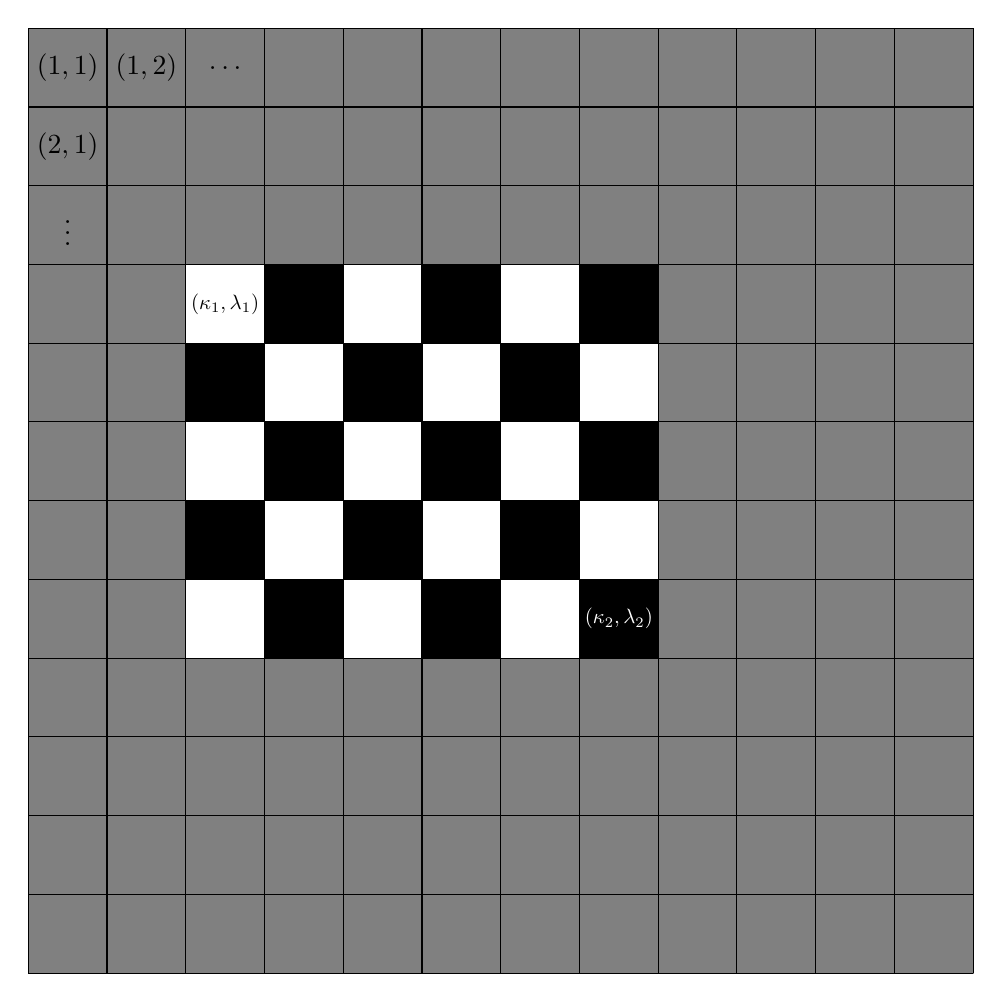
\begin{tikzpicture}
		\foreach \i in {-6, ..., 5}
			\foreach \j in {-6, ..., 5}
				\filldraw[gray] (\i, \j) rectangle + (1, 1);
		\foreach \i in {-4, ..., 1}
			\foreach \j in {-2, ..., 2}
			{
				\pgfmathparse{mod(\i+\j, 2) ? "black" : "white"}
				\edef\colour{\pgfmathresult}
				\filldraw[fill=\colour] (\i, \j) rectangle + (1, 1);
			}
		\draw[step=1] (-6, -6) grid (6, 6);
		\node at (-5.5, 5.5) {$(1, 1)$};
		\node at (-4.5, 5.5) {$(1, 2)$};
		\node at (-3.5, 5.5) {$\dots$};
		\node at (-5.5, 4.5) {$(2, 1)$};
		\node at (-5.5, 3.5) {$\vdots$};
		\node[scale=0.75] at (-3.5, 2.5) {$(\kappa_1, \lambda_1)$};
		\node[scale=0.75, white] at (1.5, -1.5) {$(\kappa_2, \lambda_2)$};
	\end{tikzpicture}
	\caption{Example of a matrix $\tilde{V}$ as in the statistical model \ref{statmodel}, that contains a ROI with a checkerboard pattern. The top left corner of the ROI is $(4, 3)$ and the bottom right corner is $(8, 8)$. Here we have $m = n = 12$.}
	\label{fig: ROI}
\end{figure}